\documentclass[12pt]{article}
\usepackage{parskip}
\usepackage{tikz}
\usepackage{amsmath}
\usepackage{amssymb}
\usepackage{graphicx}
\usepackage{minted}
\usepackage[most]{tcolorbox}
\definecolor{lightgreen}{rgb}{0.56, 0.93, 0.56}
\definecolor{moonstoneblue}{rgb}{0.45, 0.66, 0.76}
\graphicspath{{./images/}} 

\title{Traffic Light Project}

\author{Rafat Bashar}

\date{December 1, 2024}

\begin{document}
\maketitle

\section{Introduction}

\subsection{Overview}

This project involves designing and implementing a traffic light system using an Arduino Uno R3. This project is divided into three stages: blinking a single LED, blinking
two LEDs, and blinking three LEDs in a sequence that mimics a traffic light. 

There are two main goals of this project: learning how to use a programmable microcontroller, and developing documentation skills

\section{General Information}

\subsection{Materials and their Functions}

\begin{itemize}
  \item \textbf{Arduino Uno R3}
  \begin{itemize}
    \item The Arduino Uno R3 is a microcontroller board capable of performing a wide range of tasks, from turning on an LED to adding voice automation to household lighting.
    To use it, simply download the Arduino IDE onto a laptop or computer, write code in the IDE, connect the Arduino via the provided USB cord, upload the code, and watch
    the Arduino execute the code. In this project, I will use an Arduino Uno R3 to make LEDs light up in a sequence that mimics a traffic light.
  \end{itemize}
  \item \textbf{Breadboard}
  \begin{itemize}
    \item A breadboard is a platform used to create circuits without soldering components together. Because components can be easily connected and removed, breadboards allow 
    beginners to experiment with and test various circuit designs. In this project, I will use a breadboard to connect the Arduino Uno R3, LEDs, resistors, and jumper 
    cables to create a system of LEDs that functions like a traffic light, where the LEDs switch between green, yellow, and red at different intervals
  \end{itemize}
  \item \textbf{LEDs}
  \begin{itemize}
    \item An LED, or light-emitting diode, is a semiconductor device that emits light when an electric current passes through it. Although the end product of this project 
    is meant to be a traffic light system, I only have red LEDs available, so the traffic light will be monochrome.
  \end{itemize}
  \item \textbf{Resistors}
  \begin{itemize}
    \item A resistor limits the flow of current by converting electrical energy into heat energy as the current passes through it. This process results in a voltage drop in the circuit.
  \end{itemize}
  \item \textbf{Jumper Cables}
  \begin{itemize}
    \item Jumper cables are wires used to create electrical connections between components of a circuit. In this project, they will survive two primary purposes: power distribution
    and grounding. 
    \begin{itemize}
      \item \textbf{Power Distribution}: Jumper cables will transfer voltage from the Arduino's power pins to the breadboard, establishing an electrical current in the circuit. 
    \end{itemize}
    \begin{itemize}
      \item \textbf{Grounding}: Jumper cables will connect the Arduino's GND pin to the Breadboard's negative rail, providing a common ground for the entire circuit. 
    \end{itemize}
  \end{itemize}
\end{itemize}


\subsection{Physics Principles}

The most fundamental principle of physics that we should know when talking about circuits, is Ohm's Law, which describes the relationship between voltage (V), current (I), and resistance (R):


\begin{equation}
  V=IR
\end{equation}
By knowing the voltage supplied by the Arduino (in our case, this is 5V), the forward voltage of the LED (typically between 1.8-3.3V), and the forward current for the LEDs (about 10-30mA), we can calculate the required resistance to ensure the circuit works properly. Having the right amount of resistance is essential to ensuring no components are damaged; if there is too much resistance, the LED will not light up, but if there is too little resistance, the LED will draw too much current and quickly burn out. 
By plugging our known values into the equation, we get
\begin{equation}
  V_{\textrm{Source}}-V_{\textrm{LED}}=IR \rightarrow R=\frac{V_{\textrm{Source}}-V_{\textrm{LED}}}{I} \rightarrow R=\frac{5-2}{0.02}=150\Omega
\end{equation}


Although the resistors I have are 220 Ohms, the difference in Ohms between what I have and what is desired (220 and 150) is not big enough to prevent the LED from lighting up. 


Another important concept is signal flow. In this project, the signal will begin from the Arduino, which will send a digital HIGH or LOW signal to the system through a jumper cable that is connected from the Arduino to the breadboard. A HIGH signal at an output pin would complete the circuit by allowing current to flow into the breadboard, through the LED and its associated resistor to ground. A LOW signal disconnects the circuit, turning the LED off. The switching between HIGH and LOW is controleld by the code that is uploaded to the Arduino, dictating both the sequence and the timing of LEDs blinking. 


By applying both of these principles to the project, we will be able to design a system of LEDs that operates similarly to a traffic light, where one led flashes for a certain time, then, when that LED stops, another LED flashes for a set time, and finally, after that LED stops, the last LED will light up for a specified time, and then the loop will repeat. 


\section{Single LED}


\subsection{Component List}

\begin{itemize}
\item Arduino Uno R3
\item Breadboard
\item One LED
\item One 220 Ohm Resistor
\item Two Jumper Cables
\end{itemize}

\subsection{Circuit Diagram}
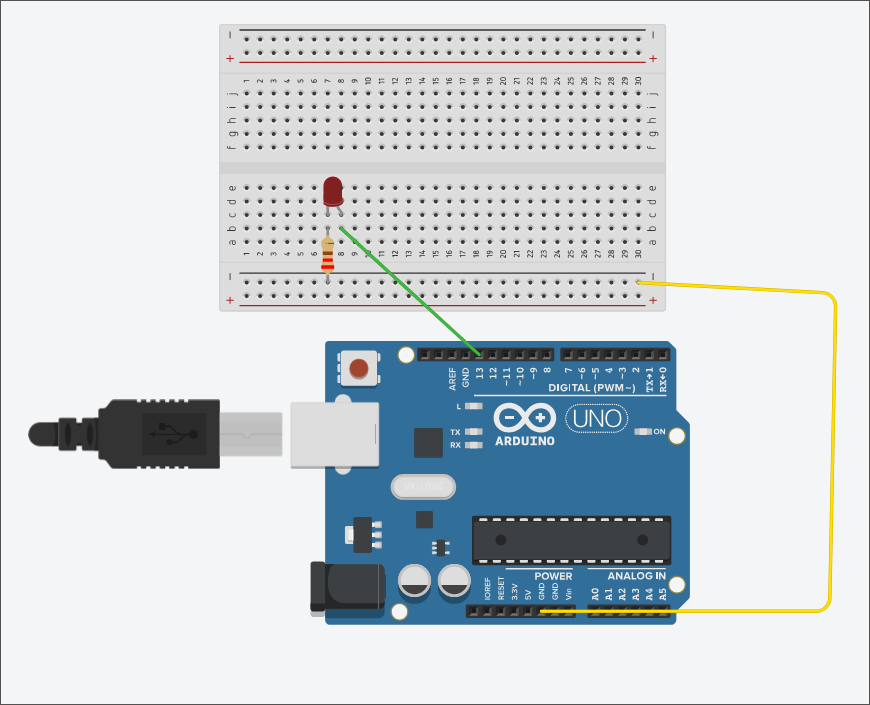
\includegraphics[width=1.0\textwidth]{One_LED_Diagram.png}
As shown in this image, I have the two jumper cables connected to the Arduino; one is connected from the ground pin to the negative rail of the breadboard, while the other is connected from Pin 13 of the Arduino to the main circuit of the breadboard. This then connects to the LED above it, and afterwards goes through the resistor, which is connected to the negative rail. The current then goes through the negative rail, into the jumper cable, and gets grounded by the Arduino. 


\subsection{Physical Setup}
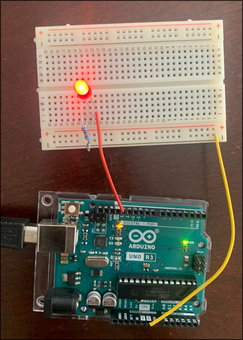
\includegraphics[width=1.0\textwidth]{PhysicalSingleLED.png}
I was able to get the LED to blink according to the code


\subsection{Development Process}
\begin{tcolorbox}[
    enhanced,
    attach boxed title to top left={xshift=6mm,yshift=-3mm},
    colback=lightgreen!20,
    colframe=lightgreen,
    colbacktitle=lightgreen,
    title=Code for Single LED,
    fonttitle=\bfseries\color{black},
    boxed title style={size=small,colframe=lightgreen,sharp corners},
    sharp corners,
]
\begin{minted}[linenos]{cpp}
int GREEN = 13;

void setup() {
 
  pinMode(GREEN, OUTPUT);
}

void loop(){
  digitalWrite(GREEN, HIGH);
  delay(5000);
  DigitalWrite(GREEN, LOW);
  delay(5000);

}

\end{minted}
\end{tcolorbox}

At first I tried running the program without any delay, but this caused the light to appear as if it never turned off. This is because the voltage was switching between 
HIGH and LOW so fast that it seemed as though the light was constantly on. The first line of code labels Pin 13 on the Arduino as GREEN to represent the green LED in the 
system. In the setup section, I specify which pins of the Arduino will act as outputs; these are the pins used to control the current by turning it on and off. 
In the loop section, I start by turning on the current to the green LED by setting the GREEN (Pin 13) output to HIGH. After that, there's a 5000ms (five second) delay, 
so the Arduino waits five seconds before executing the next line of code, which turns off the current. Then, I added one last five-second delay before the code loops 
back to the beginning. This makes it so that the LED stays off for five seconds, and then, after looping back to the beginning, the LED turns back on, creating a 
blinking pattern with 5 second on-off intervals. 

\section{Two LEDs}

\subsection{Component List}

\begin{itemize}
\item Arduino Uno R3
\item Breadboard
\item Two LEDs (Added One)
\item Two 220 Ohm Resistors (Added One)
\item Three Jumper Cables (Added One)
\end{itemize}

\subsection{Circuit Diagram}
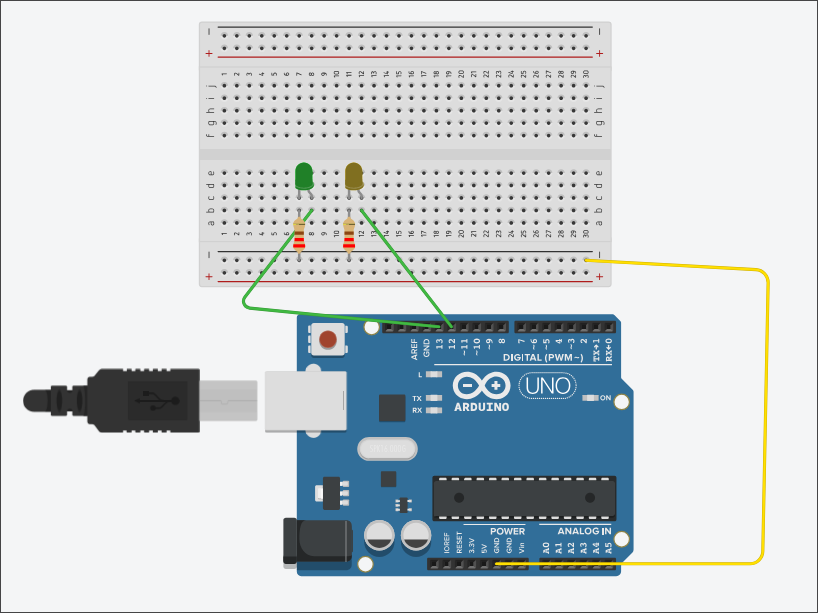
\includegraphics[width=1.0\textwidth]{Two_LED_Diagram.png}

\subsection{Physical Setup}
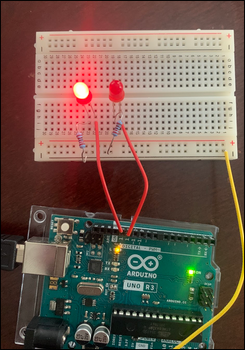
\includegraphics[width=0.5\textwidth]{PhysicalTwoLEDOne.png}
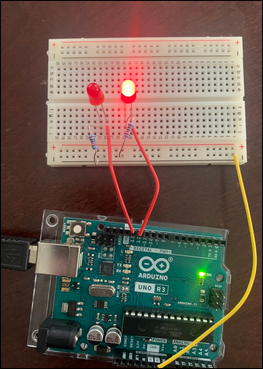
\includegraphics[width=0.5\textwidth]{PhysicalTwoLEDTwo.png}
I successfully got two LEDs to blink in an alternating order (The one on the left should be green, and the one on the right should be yellow)

\subsection{Development Process}
\begin{tcolorbox}[
    enhanced,
    attach boxed title to top left={xshift=6mm,yshift=-3mm},
    colback=lightgreen!20,
    colframe=lightgreen,
    colbacktitle=lightgreen,
    title=Code for Two LEDs,
    fonttitle=\bfseries\color{black},
    boxed title style={size=small,colframe=lightgreen,sharp corners},
    sharp corners,
]
\begin{minted}[linenos]{cpp}
int GREEN = 13;
int YELLOW = 12;

void setup() {
 
  pinMode(GREEN, OUTPUT);
  pinMode(YELLOW, OUTPUT);
}

void loop(){
  digitalWrite(GREEN, HIGH);
  delay(5000);
  DigitalWrite(GREEN, LOW);
  digitalWrite(YELLOW, HIGH);
  delay(2000);
  DigitalWrite(YELLOW, LOW);
}
\end{minted}
\end{tcolorbox}
The main difference between this code and the code for a single LED is how the transitions are done. Specifically, after turning the GREEN output to LOW, there's no delay
before turning the YELLOW output to HIGH. This mimics how traffic lights work. There isn't a pause; when the green light is done, it immediately switches to yellow. 
I decided to make the yellow light last two seconds only, hence the 2000ms delay. When the YELLOW output is put to LOW, the code loops back and instantly turns the GREEN 
output to high.

\section{Traffic Lights}

\subsection{Component List}

\begin{itemize}
\item Arduino Uno R3
\item Breadboard
\item Three LEDs (Added Another One)
\item Three 220 Ohm Resistor (Added Another One)
\item Four Jumper Cables (Added Another One)
\end{itemize}


\subsection{Circuit Diagram}
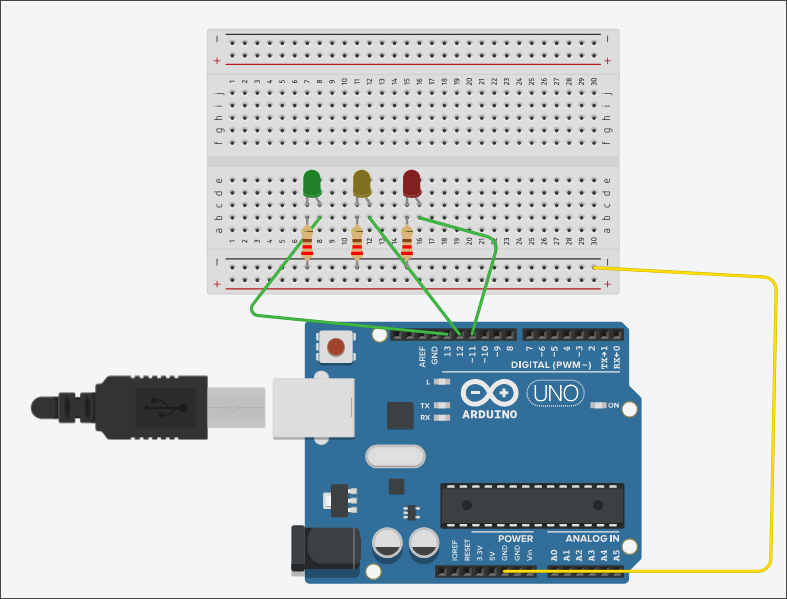
\includegraphics[width=1.0\textwidth]{Three_LED_Diagram.png}

\subsection{Physical Setup}
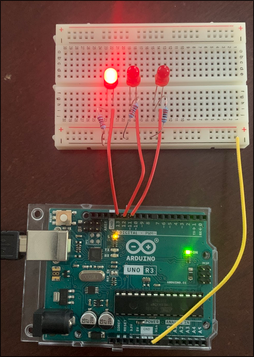
\includegraphics[width=0.33\textwidth]{PhysicalTrafficLightOne.png}
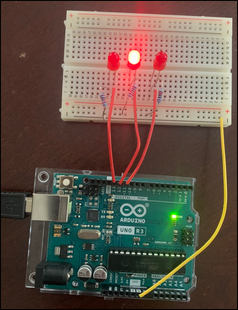
\includegraphics[width=0.33\textwidth]{PhysicalTrafficLightTwo.png}
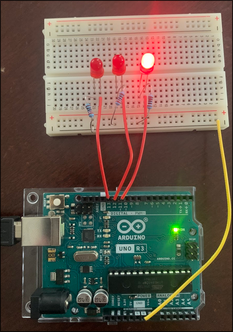
\includegraphics[width=0.33\textwidth]{PhysicalTrafficLightThree.png}
I was able to finish my LED traffic light system. In these images, the left LED should be green, the middle LED should be yellow, and the right LED should be red. 
However, the only LEDs I had were red, so I was unable to get the proper colors. Regardless, the system functions as intended. 

\subsection{Development Process}
\begin{tcolorbox}[
    enhanced,
    attach boxed title to top left={xshift=6mm,yshift=-3mm},
    colback=lightgreen!20,
    colframe=lightgreen,
    colbacktitle=lightgreen,
    title=Code for a Traffic Light,
    fonttitle=\bfseries\color{black},
    boxed title style={size=small,colframe=lightgreen,sharp corners},
    sharp corners,
]
\begin{minted}[linenos]{cpp}
int GREEN = 13;
int YELLOW = 12;
int RED = 11;

void setup() {
 
  pinMode(GREEN, OUTPUT);
  pinMode(YELLOW, OUTPUT);
  pinMode(RED, OUTPUT);
}

void loop(){
  digitalWrite(GREEN, HIGH);
  delay(5000);
  DigitalWrite(GREEN, LOW);
  digitalWrite(YELLOW, HIGH);
  delay(2000);
  DigitalWrite(YELLOW, LOW);
  digitalWrite(RED, HIGH);
  delay(4000);
  DigitalWrite(RED, LOW);
}

\end{minted}
\end{tcolorbox}
This code operates in a similar fashion to that which was used for two LEDs. The only difference is that here we have another LED to represent the red light. I decided to make this light last for 4000ms before it stops and loops back to the green light. 



\end{document}
